\chapter{Wissensgenerierung - Vorgehen}
\label{chp:procedure}
In Kapitel \ref{chp:sequences} wurden Sequenzen und ihre Eigenschaften vorgestellt. Im Folgenden wird anhand eines fiktiven Beispiels das Vorgehen zur Wissensgenerierung aus Produktionsdaten - auf Grundlage der vorgenommenen Definitionen - beschrieben. Es werden die Daten von zwei Produktionsmaschinen, welche in einer Fertigungslinie hintereinander angeordnet sind (vgl. Abbildung \ref{fig:procedure-production-line}), miteinander verglichen.

\begin{figure}[H]
	\centering
	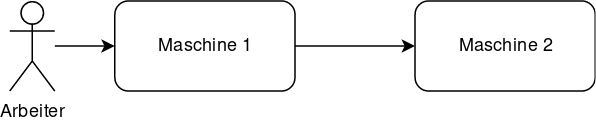
\includegraphics[scale=0.40]{images/procedure/production-line}
	\caption{Fertigungslinie mit zwei Maschinen}
	\label{fig:procedure-production-line}
\end{figure}

In diesem Beispiel wird Maschine 1 mit Stückteilen befüllt. Diese werden dort vorverarbeitet und an Maschine 2 zur Endverarbeitung weitergegeben. Eine Produktionsmaschine kann laufen, warten oder stehen. Bei der Datenerhebung wird dabei zwischen vier möglichen Zuständen unterschieden (vgl. Tabelle \ref{tab:procedure-status-in-production}). 

\begin{table}
	\begin{center}
		\begin{tabular}{|c c c|} 
			\hline
			Symbol & Zustand & Beschreibung \\
			\hline\hline
			0 & läuft & Maschine läuft im Standardbetrieb \\ 
			\hline
			1 & steht & Maschine wurde durch Mitarbeiter angehalten \\
			\hline
			2 & steht & Maschine hat von alleine angehalten \\
			\hline
			3 & wartet & Maschine wartet auf Vorgänger in Fertigungslinie \\
			\hline
		\end{tabular}
		\caption{Zustände in Fertigungslinie}
		\label{tab:procedure-status-in-production}
	\end{center}
\end{table}

In diesem Beispiel werden die erhobenen Daten zum aktuellen Zustand der beiden Maschinen für einen Tag betrachtet. Dabei wird von 16 Arbeitsstunden und einer Datenerhebung pro Minute ausgegangen, weshalb für jede Maschine 960 Datenpunkte generiert werden (vgl. Abbildung \ref{fig:procedure-raw-data}).

\begin{figure}[H]
	\centering
	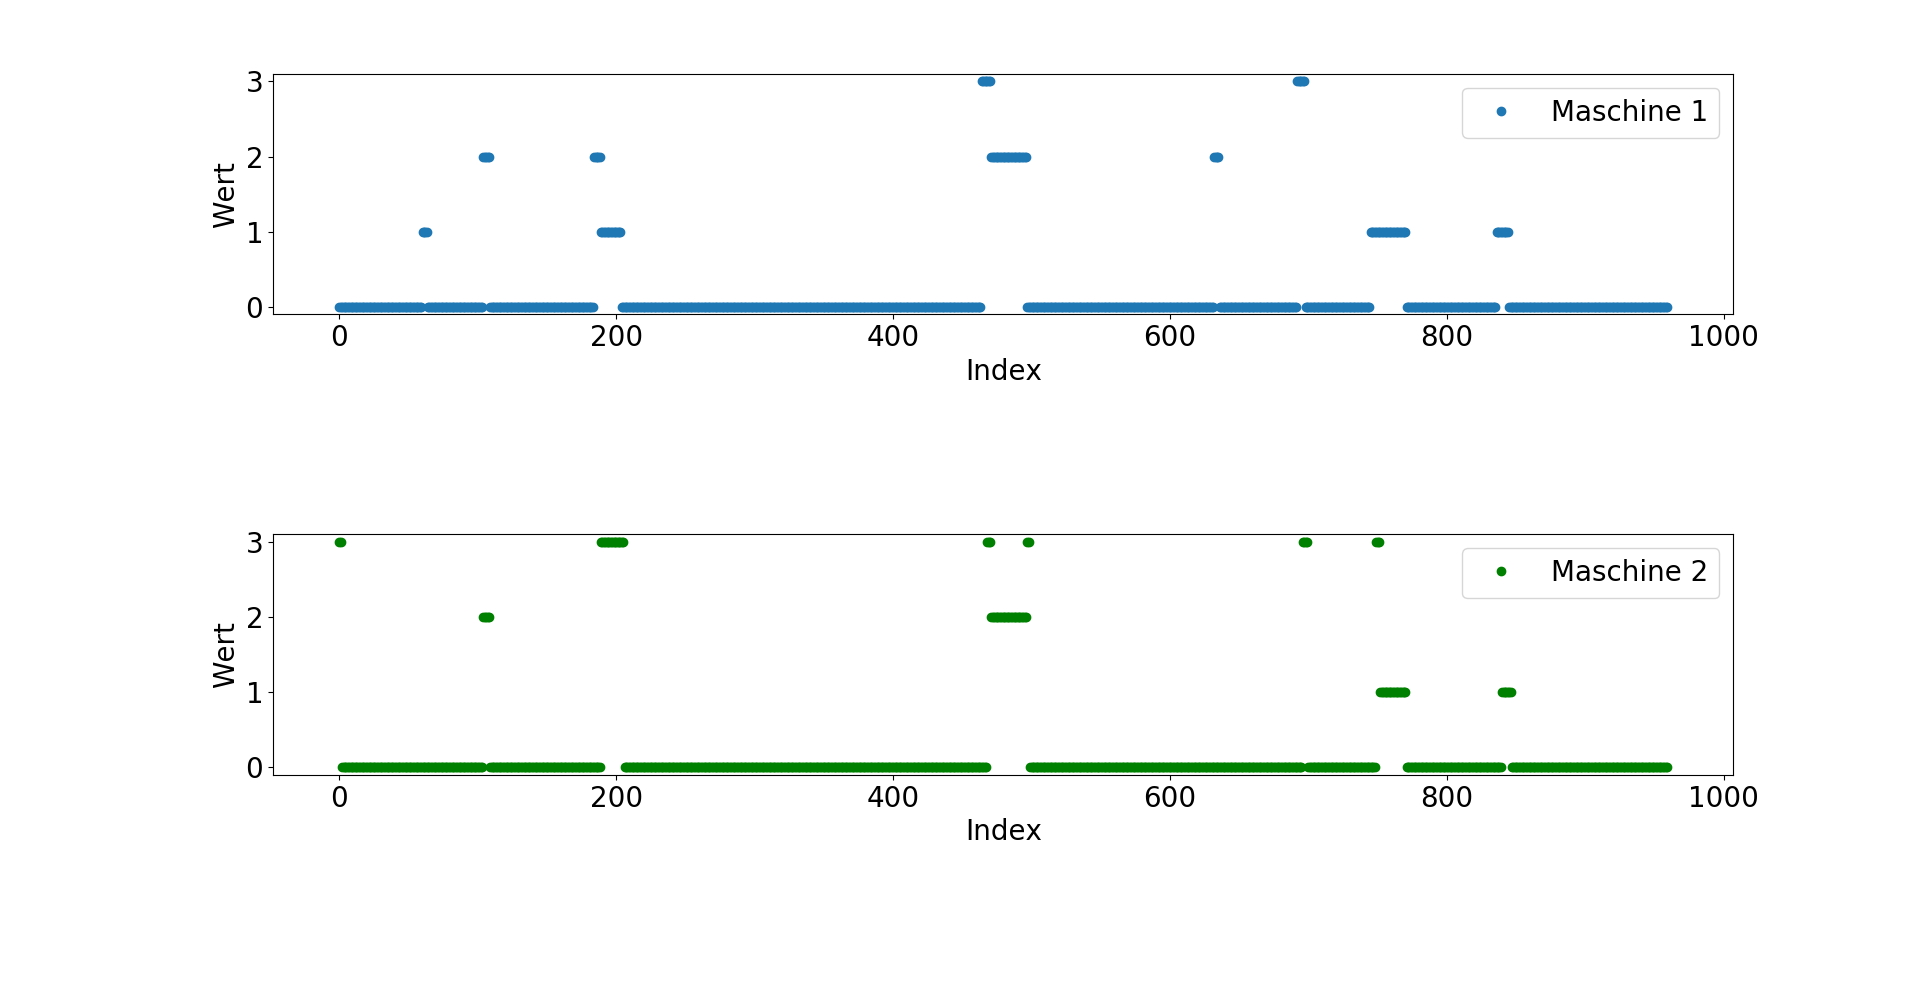
\includegraphics[scale=0.32]{images/procedure/raw-data}
	\caption{Produktionsdaten Fertigungslinie (roh)}
	\label{fig:procedure-raw-data}
\end{figure}

\section{Datenaufbereitung}
Anders als bei simulierten Daten, muss man bei Produktionsdaten mit Fehlern rechnen. So kann es schon durch einen verdreckten Sensor zu Messfehlern oder Lücken in den Messreihen kommen\footnote{ \cite{DataMining2015}}. Fehler müssen somit entfernt oder korrigiert werden. Die im Folgenden beschriebenen Schritte haben daher zur Annahme, dass eine umfassende Aufbereitung der Daten vorgenommen wurde.

Als erstes werden die Produktionsdaten auf binäre Sequenzen reduziert. Dazu müssen die Zustände (Tabelle \ref{tab:procedure-status-in-production}) in die Kategorien \textit{Fehlerzustand} und \textit{kein Fehlerzustand} aufgeteilt werden. Zur ersten Kategorie gehören dabei die Zustände 1,2 und 3, da es sich bei diesen um ein unerwünschtes Verhalten im Sinne eines reibungslosen Produktionsprozesses handelt. Der einzige fehlerfreie Zustand bleibt die 0 (vgl. Tabelle \ref{tab:procedure-reduced-status-in-production}).

\begin{table}
	\begin{center}
		\begin{tabular}{|c c c|} 
			\hline
			Symbol & Zustand & Beschreibung \\
			\hline\hline
			0 & kein Fehlerzustand & Maschine läuft im Standardbetrieb \\ 
			\hline
			1 & Fehlerzustand & Maschine wartet oder wurde durch Mitarbeiter / von selbst angehalten  \\
			\hline
		\end{tabular}
		\caption{Reduzierte Zustände in Fertigungslinie}
		\label{tab:procedure-reduced-status-in-production}
	\end{center}
\end{table}

Bei diesem Arbeitsschritt zeigt sich, dass es bereits schwierig sein kann die ursprünglichen Zustände auf zwei zu reduzieren. In diesem Beispiel könnte der Zustand \textit{wartet} (Tabelle \ref{tab:procedure-status-in-production}) auch als \textit{kein Fehlerzustand} gewertet werden, da das Warten einer Maschine an sich kein Fehlverhalten ist. Hier wird er allerdings als \textit{Fehlerzustand} gewertet, da es in dieser Fertigungslinie Abhängigkeiten der Maschinen untereinander gibt. Daher kann bspw. das Warten von Maschine 2 auf einen Fehler von  Maschine 1 zurückgeführt werden.

Wenn man das Ergebnis der Datenaufbereitung visualisiert (Abbildung \ref{fig:procedure-reduced-data}), zeigt sich die gewünschte Vereinfachung auf zwei Zustände.

\begin{figure}[H]
	\centering
	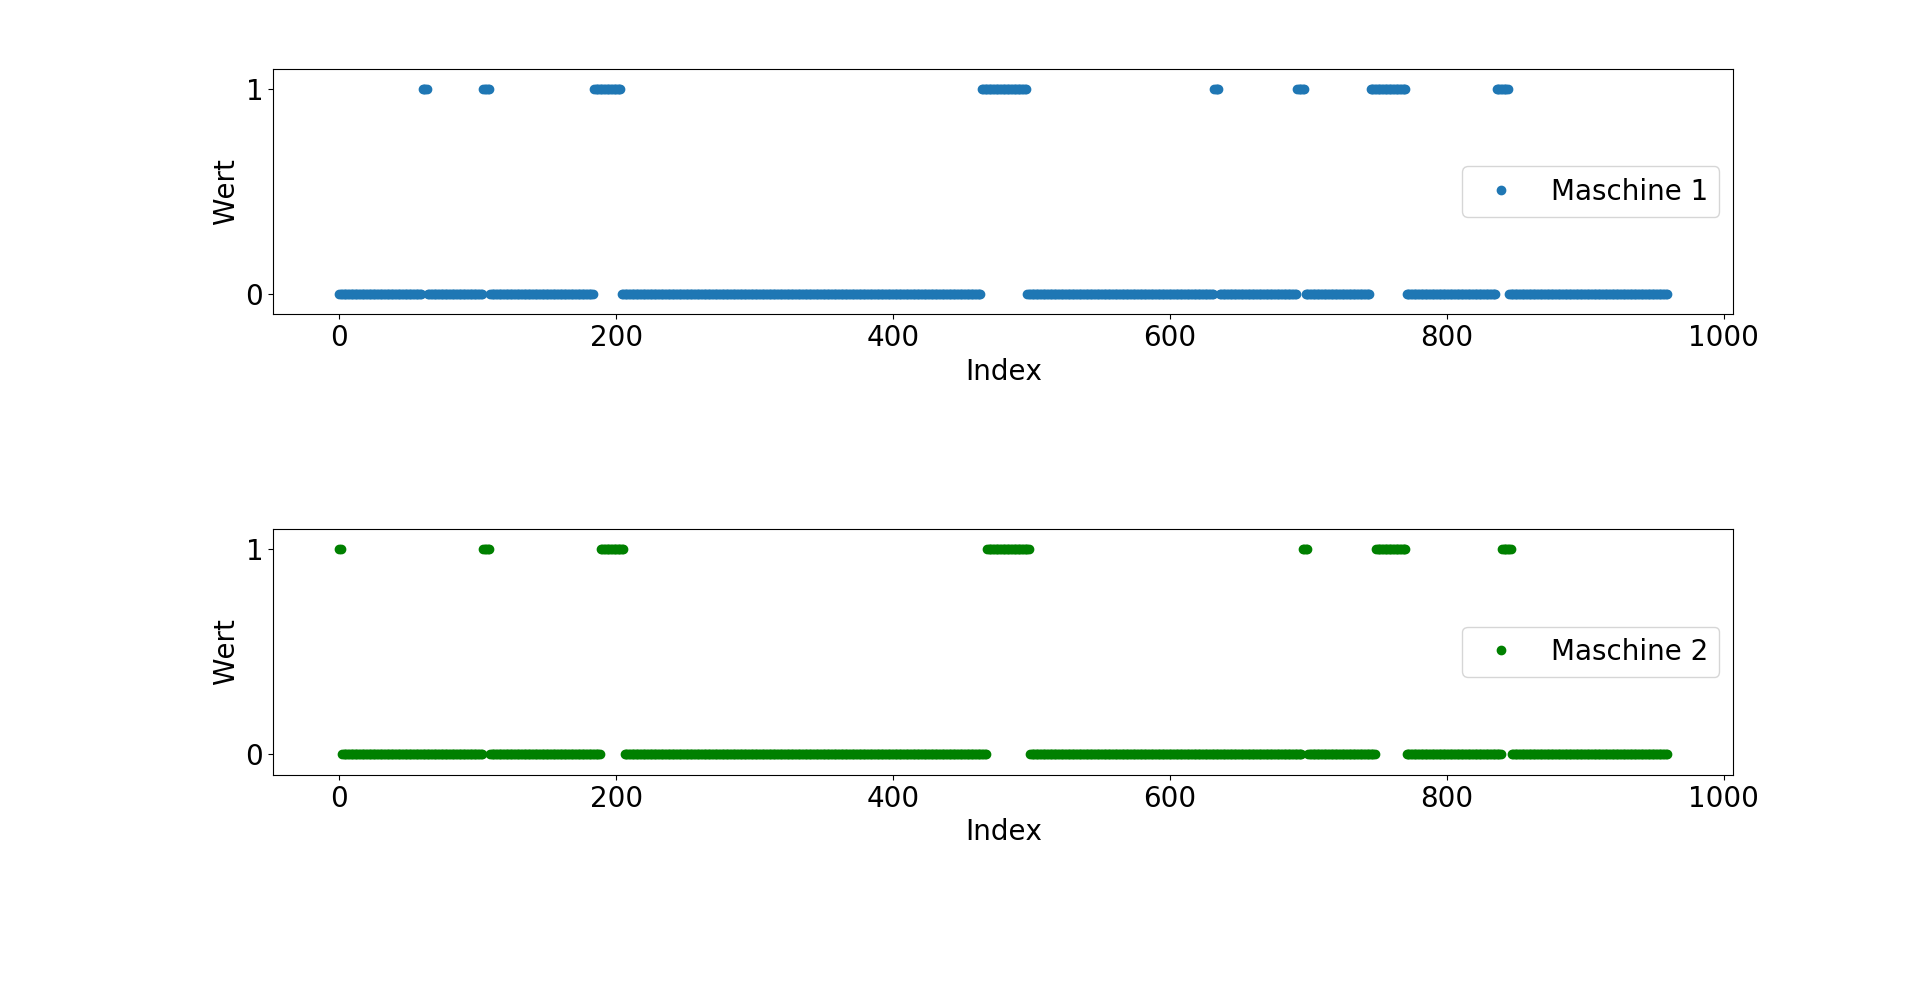
\includegraphics[scale=0.32]{images/procedure/reduced-data}
	\caption{Produktionsdaten Fertigungslinie (reduziert)}
	\label{fig:procedure-reduced-data}
\end{figure}

\section{Analyse}

\subsubsection{Balance und Frequenz}

Die Klassifizierung beginnt damit, dass die Balance ($B(1)$) und Frequenz für beide Sequenzen nach \ref{eq:properties-sequences-balance} und \ref{eq:properties-sequences-frequency} berechnet werden.
\begin{itemize}
	\item $Balance_{M1} = 0.11$
	\item $Balance_{M2} = 0.09$
	\item $Frequenz_{M1} = 0.02$
	\item $Frequenz_{M2} = 0.01$
\end{itemize}
Auch wenn diese Werte noch keine große Aussagekraft haben, lässt sich durch sie zumindest der Eindruck einer visuellen Betrachtung (Abbildung \ref{fig:procedure-reduced-data}) bestätigen. Die Balance ist für beide Maschinen unausgeglichen. Maschine 1 befand sich über den ganzen Tag zu 11\% und Maschine 2 zu 9\% der Zeit in einem fehlerhaften Zustand. Beide Maschinen sind zudem mit 0.02 und 0.01 sehr niederfrequent.

Der nächste Schritt ist eine feinere Betrachtung der bekannten Eigenschaften. Dazu werden die Balance und Frequenz für Teilsequenzen der Länge 10 berechnet. Somit lassen sich aus den 960 Datenpunkten 96 Werte für Balance und Frequenz erzielen. Die Ergebnisse sind in den Abbildungen \ref{fig:procedure-balance-machine-1-subsequence} und \ref{fig:procedure-balance-machine-2-subsequence} für die Balance sowie in \ref{fig:procedure-frequency-machine-1-subsequence} und \ref{fig:procedure-frequency-machine-2-subsequence} für die Frequenz dargestellt.

\begin{figure}[H]
	\centering
	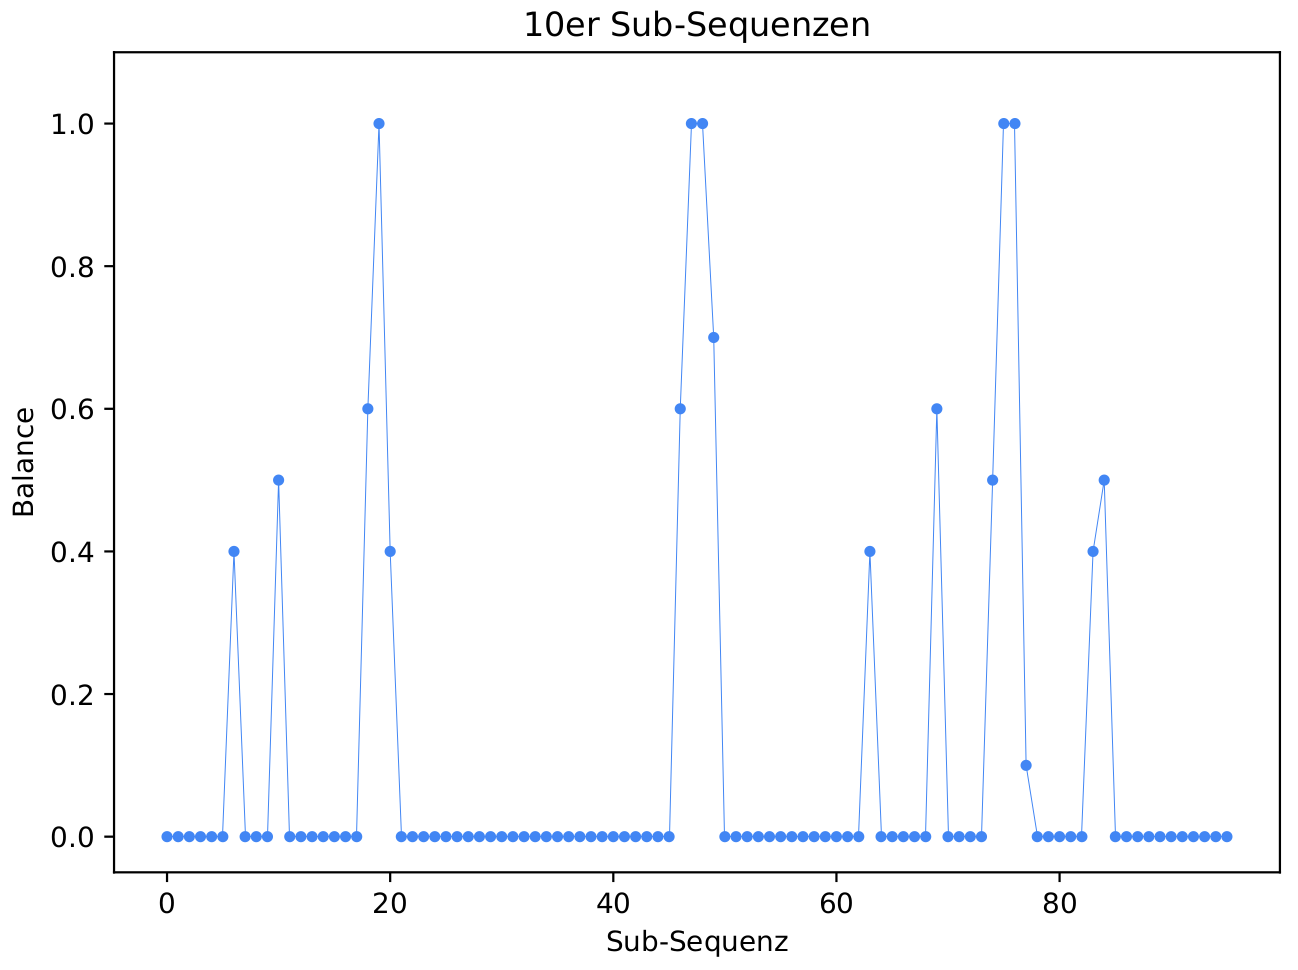
\includegraphics[scale=0.20]{images/procedure/balance_machine_1}
	\caption{Maschine 1: Balance der 10er Subsequenzen}
	\label{fig:procedure-balance-machine-1-subsequence}
\end{figure}

\begin{figure}[H]
	\centering
	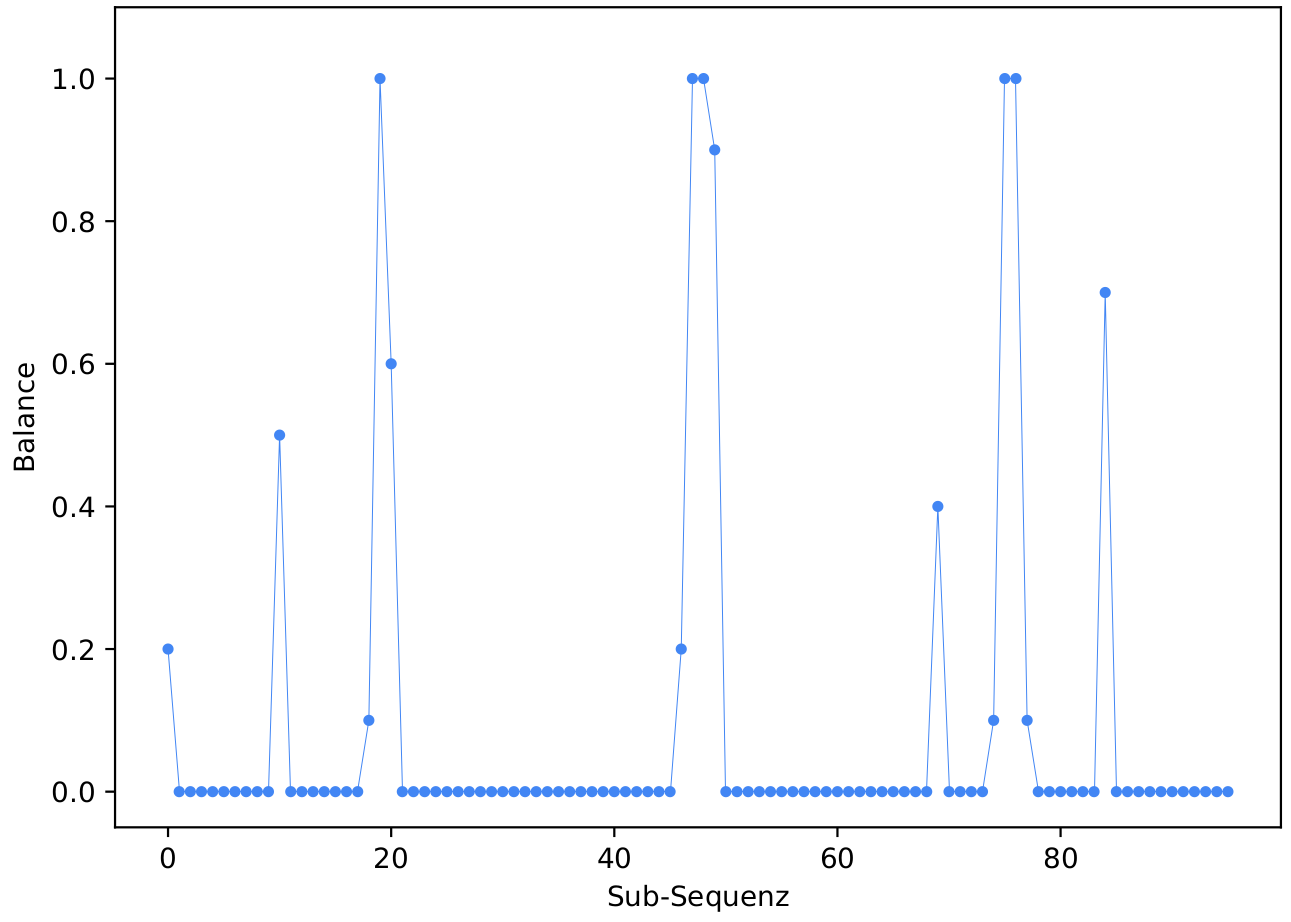
\includegraphics[scale=0.20]{images/procedure/balance_machine_2}
	\caption{Maschine 2: Balance der 10er Subsequenzen}
	\label{fig:procedure-balance-machine-2-subsequence}
\end{figure}

\begin{figure}[H]
	\centering
	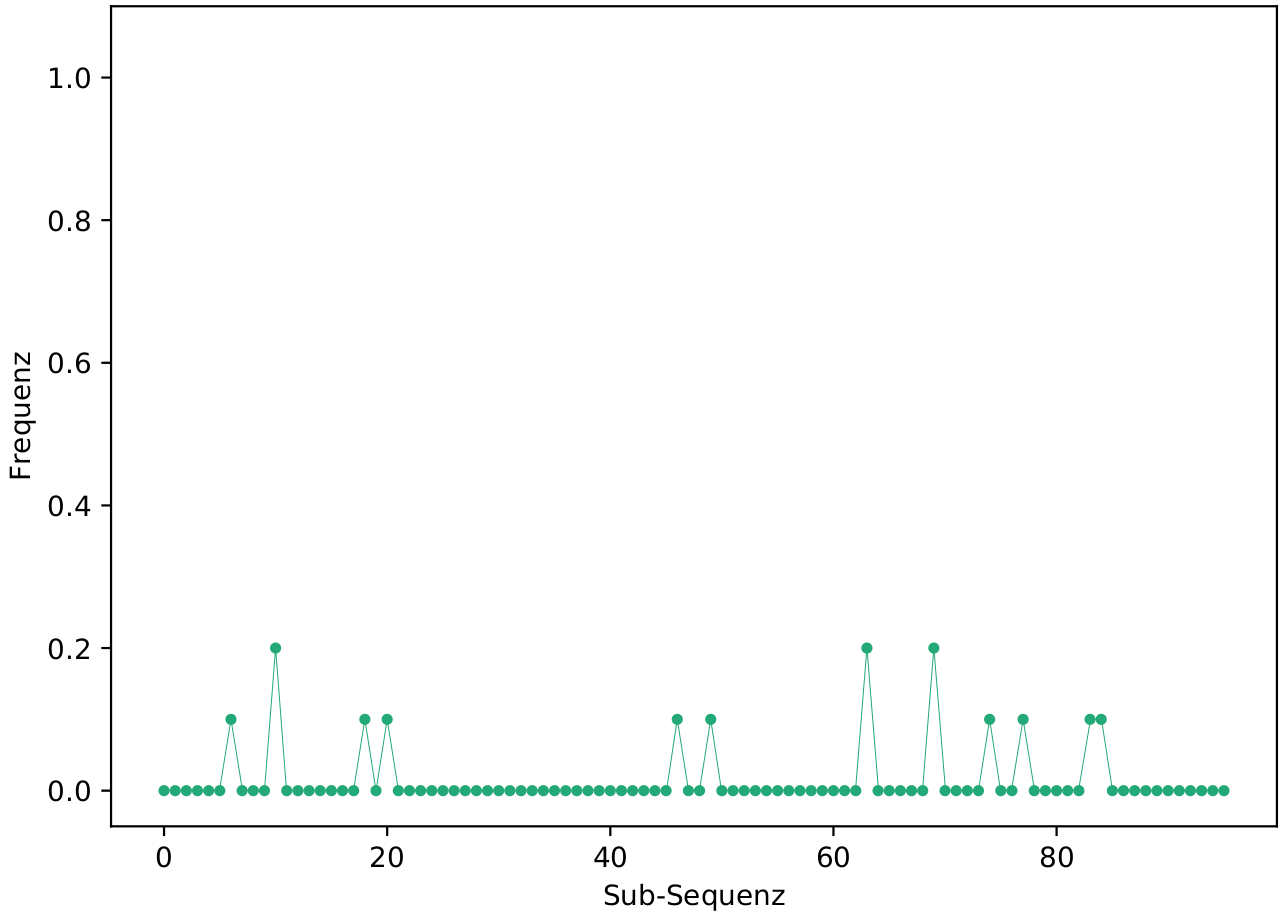
\includegraphics[scale=0.20]{images/procedure/frequency_machine_1}
	\caption{Maschine 1: Frequenz der 10er Subsequenzen}
	\label{fig:procedure-frequency-machine-1-subsequence}
\end{figure}

\begin{figure}[H]
	\centering
	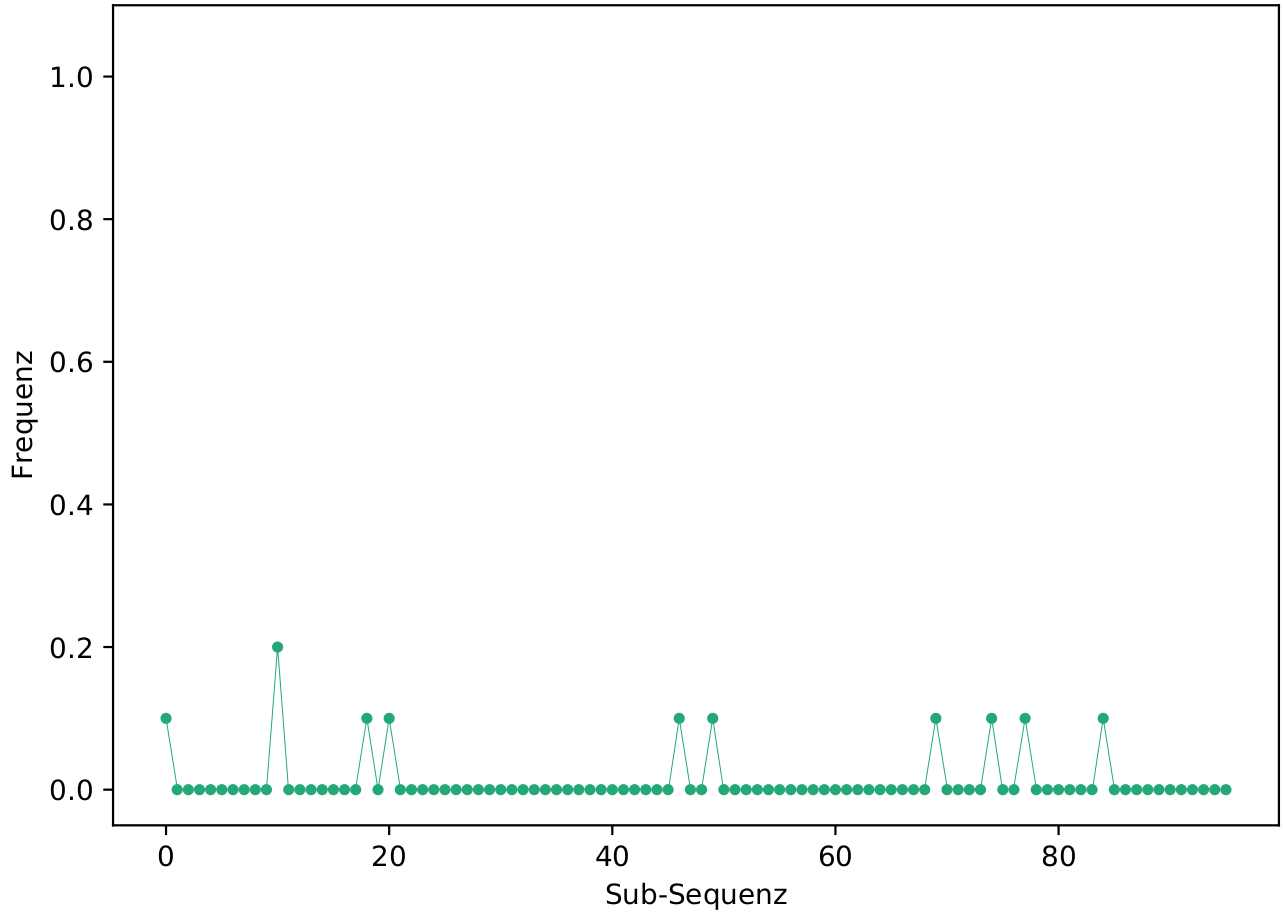
\includegraphics[scale=0.20]{images/procedure/frequency_machine_2}
	\caption{Maschine 2: Frequenz der 10er Subsequenzen}
	\label{fig:procedure-frequency-machine-2-subsequence}
\end{figure}

Beim Vergleichen der Balance und Frequenz der beiden Maschinen untereinander zeigen sich die Ähnlichkeiten der Plots zueinander. Dabei auffällig ist ein auftretendes Muster bei der Balance von Maschine 1 (vgl. Abbildung \ref{fig:procedure-balance-machine-1-subsequence}), dass beides Mal für mindestens 10 Minuten ausschließlich in einem Fehlerzustand ist. Das Muster findet sich von Index 6 bis 9 und 62 bis 77. In Abbildung \ref{fig:procedure-balance-machine-2-subsequence} zeigt sich ebenfalls ein Muster von 10 bis 19 und 68 bis 77, welches sich jeweils mindestens 10 Minuten ausschließlich im Fehlerzustand befindet.

Die Frequenz beider Maschinen weist ebenfalls ein repetitives  Muster auf. So ist dieses bei beiden Maschinen von 17 bis 21, 45 bis 50 und 73 bis 78 zu beobachten (vgl. Abbildungen \ref{fig:procedure-frequency-machine-1-subsequence} und \ref{fig:procedure-frequency-machine-2-subsequence}).

Zusammenfassend lässt sich sagen, dass eine zeitliche Korrelation zwischen den Maschinen zu beobachten ist. Entsprechend würde sich hier die Anwendung der Kreuzkorrelationsfunktion zur Verifikation empfehlen.



\subsubsection{Korrelation}

Mit dem Tool aus Kapitel \ref{chp:crosscorrelation:implementation} erhalten wir das Ergebnis, welches in Abbildung \ref{fig:procedure-crosscorrelation-subsequence} abgebildet ist.

\begin{figure}[H]
	\centering
	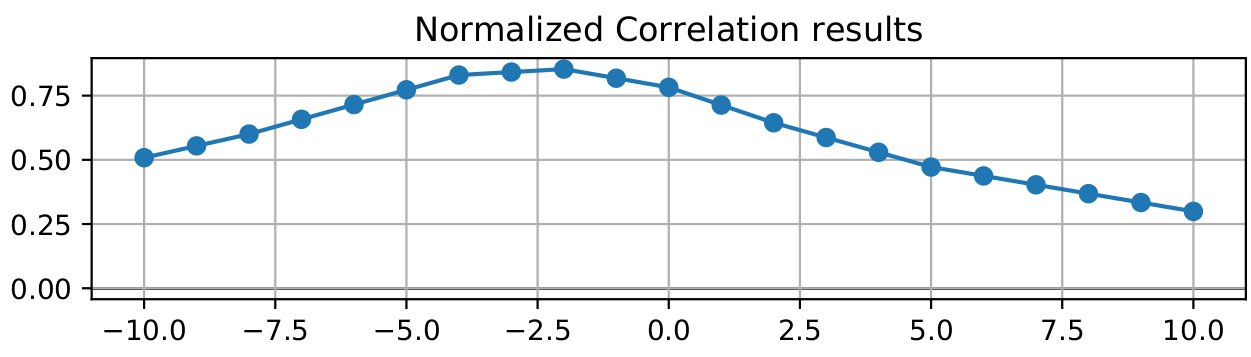
\includegraphics[scale=0.32]{images/procedure/crosscorrelation_machine_1_machine_2}
	\caption{Kreuzkorrelation}
	\label{fig:procedure-crosscorrelation-subsequence}
\end{figure}

Das Ergebnis der Auswertung bestätigt die erste Vermutung, dass eine zeitliche Korrelation zwischen beiden Maschinen besteht. Das Maximum von ca. $0.8$ der normalisierten Kreuzkorrelation liegt ungefähr zwischen $-2.5$ und $-2.0$ und stellt die Verschiebung dar. Dieses Ergebnis lässt sich so deuten, dass Maschine 2 um den Verschiebungswert auf der x-Achse nach rechts verschoben ist. Das bedeutet, dass Maschine 1 meistens vor Maschine 2 in den \textit{Fehlerzustand} springt. Somit lässt sich der erste Eindruck mit der Kreuzkorrelationsfunktion bestätigen.